\subsection{Logan Montgomery}
My immediate tangible goal is to get use to being retired (27 July).  Next, I want to complete my second M.S. in Computer Science.  Following my second M.S., I want to pursue a PhD in Computer Science, gain meaningful employment as a University Professor, and continue research in various domains impacted by or dependent on computer science.  Intangibly, “I am a lifelong learner.”  I do not have an objective or completion date for my journey through curiosity, education, and research.  My goal is simple, “breath, engage in life, learn, and influence change where possible.”

\begin{figure}[ht]
	\centering
    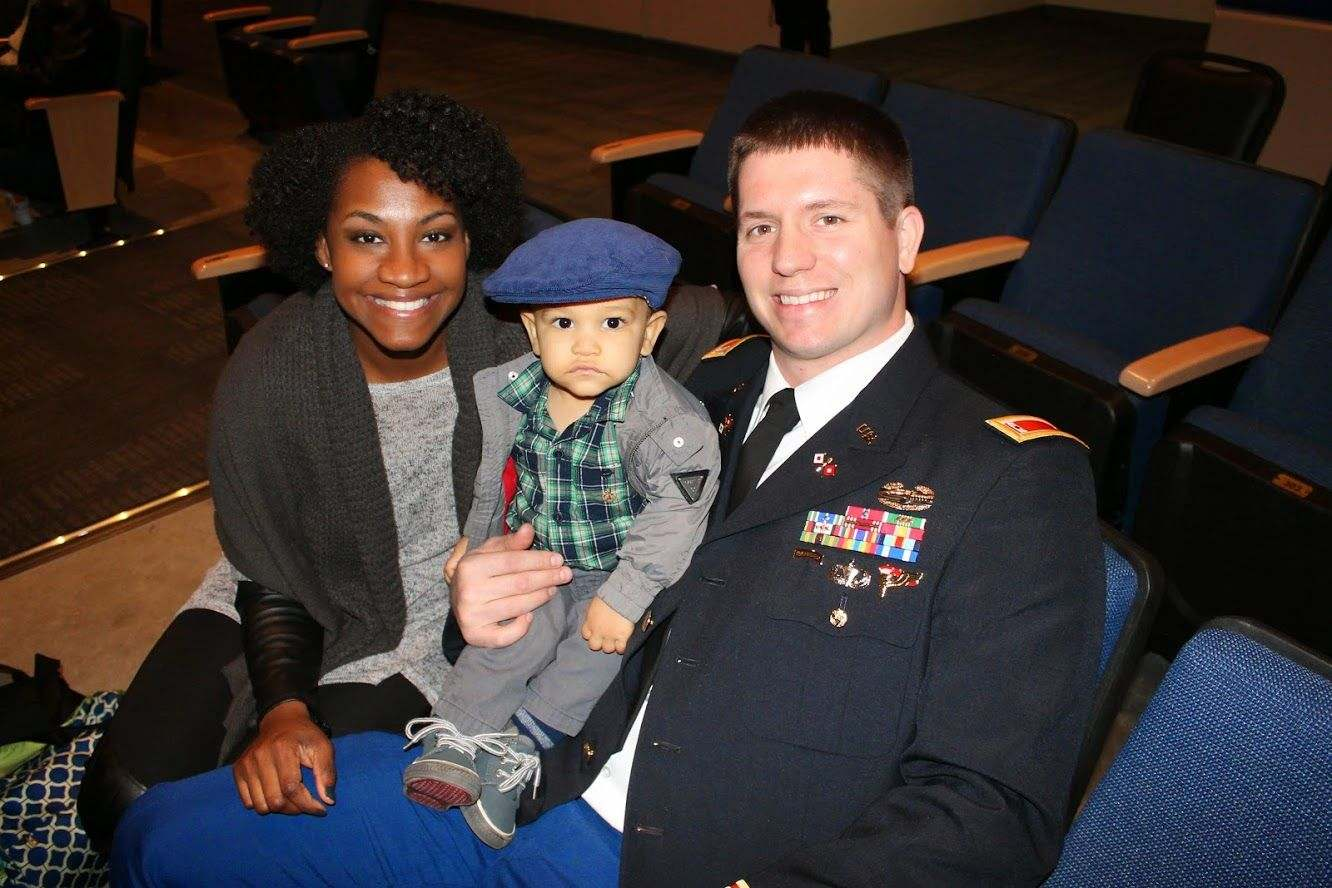
\includegraphics[width=3in]{myimage}
    \caption{My Family and I}
    \label{fig:My Family and I}
\end{figure}

\subsection{Related GIT - Covert Channel Through TCP Checksums Using SCAPY}
I chose a random covert channel git repo.  I don't have a research area officially, but I play around with network security and data exfiltration techniques regularly.  So, I though I'd share a pretty straight forward method of transferring data by crafting TCP checksums using SCAPY.   

\url{https://github.com/mtarsel/Covert-Channel}